%!TEX root = ../paper.tex

\subsubsection{Data Type}
\label{sec:datatypes}

Based on our data, we observed that the largest effect stemmed from the data being shared. We present various statistical models in section \ref{sec:regression} to support this conclusion. The most and least concerning data are listed in Table \ref{top10-table}, and the full list of data can be seen in Appendix \ref{sec:data-appendix}. 

Participants were most concerned about photos and videos, especially if they contained embarrassing content, nudity, or financial information. As seen in Table \ref{top10-table}, photos and videos accounted for five of the top ten concerns, and are almost unanimously considered to be concerning. Information that could be used to impersonate someone (e.g., usernames/passwords for websites) or invade privacy (photos of someone at home) were also among the most concerning data types. 

Participants were least concerned about data that could be observed through observations of public behavior, such as demographic information (e.g., age, gender, language spoken) and information available to advertisers (e.g. TV shows watched, music on device). As seen in Table \ref{top10-table}, participants had spread distributions in perceptions regarding such information.  These may have appeared as unconcerning because of unfamiliarity in what applications would use this data for, or because there does not seem to be any immediate financial, social, or physical consequences from having this shared.

Although certain data is considered unanimously upsetting to have shared, it is interesting to note that no data was considered unanimously non-upsetting to have shared, nor any data which evoked strong disagreement on how upsetting it was. Generally,  the rank of the data being shared is negatively correlated with the standard deviation of the answers. For the complete ranked list of data considered in this study, see Appendix \ref{sec:data-appendix}.

\begin{table*}[t]
\begin{center}
\small
\begin{tabular}{| r | l | r | r |c |}
\hline
Rank & Data & VUR & $\sigma$ & Distribution \\
\hline
1 & video of you unclothed & 95.97\% & 0.31 & 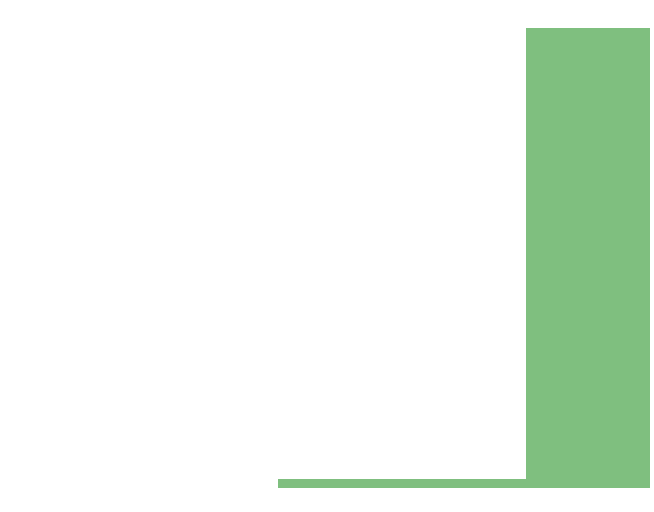
\includegraphics[width = 2cm, height = 0.5cm]{tex-inputs/data10/tookavideoofyouunclothedcombined} \\
2 & bank account information & 95.91\% & 0.35 & 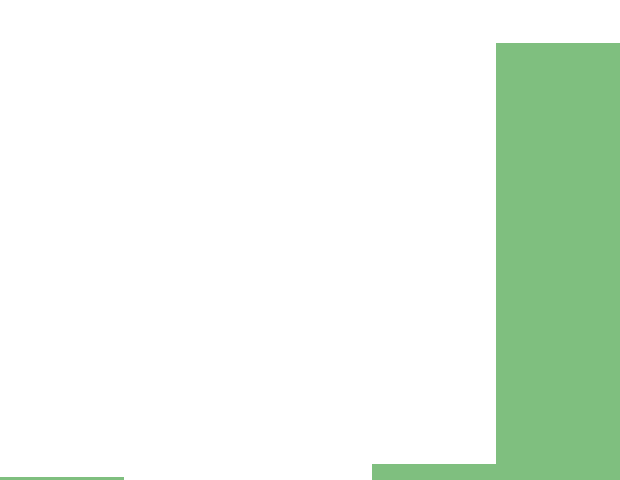
\includegraphics[width = 2cm, height = 0.5cm]{tex-inputs/data10/learnedyourbankaccountinformationcombined}  \\
3 & social security number & 94.84\% & 0.26 & 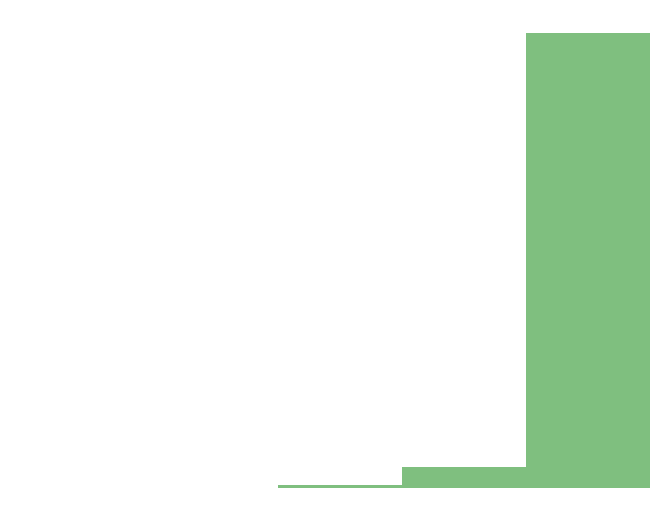
\includegraphics[width = 2cm, height = 0.5cm]{tex-inputs/data10/learnedyoursocialsecuritynumbercombined}\\
4 & video entering in a PIN at an ATM & 92.67\% & 0.47 & 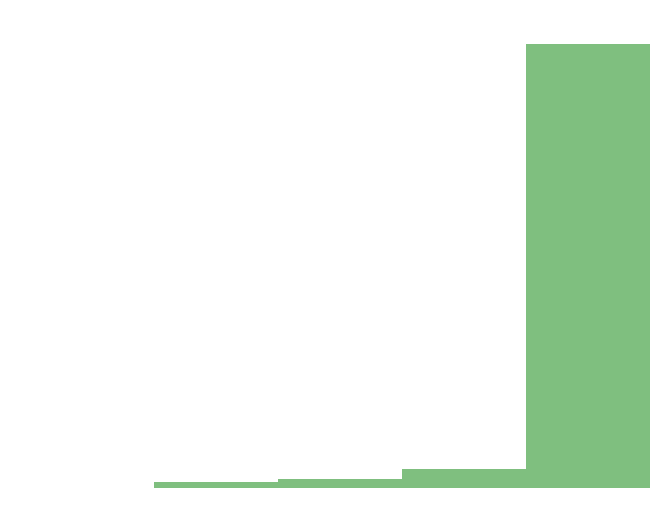
\includegraphics[width = 2cm, height = 0.5cm]{tex-inputs/data10/tookavideoofyouenteringinyourPINatanATMcombined}\\
5 & photo of you unclothed & 92.59\% & 0.46 & 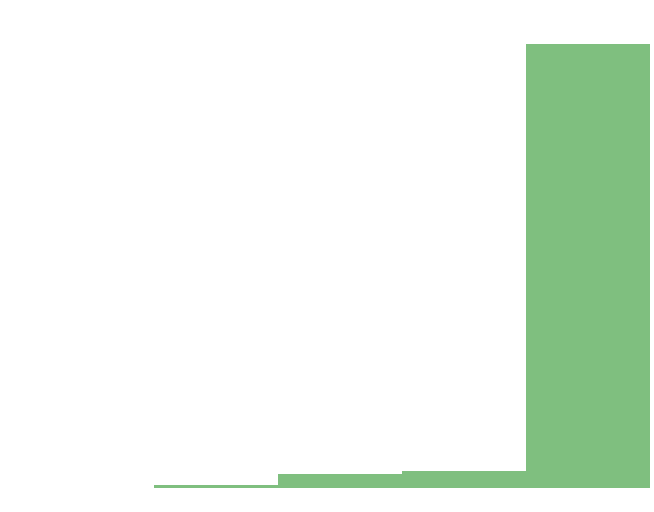
\includegraphics[width = 2cm, height = 0.5cm]{tex-inputs/data10/tookaphotoofyouunclothedcombined}\\
6 & photo of you that is very embarrassing & 91.39\% & 0.55 & 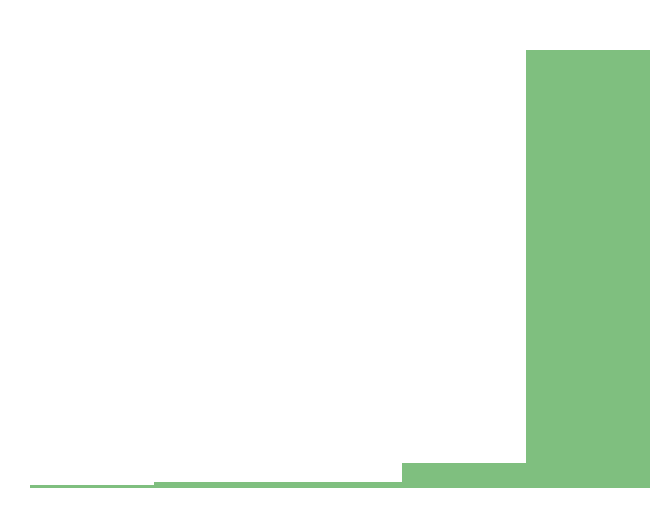
\includegraphics[width = 2cm, height = 0.5cm]{tex-inputs/data10/tookanincriminatingphotoofyoudoingsomethingembarrassingcombined}\\
7 & username and password for websites & 89.55\% & 0.62 & 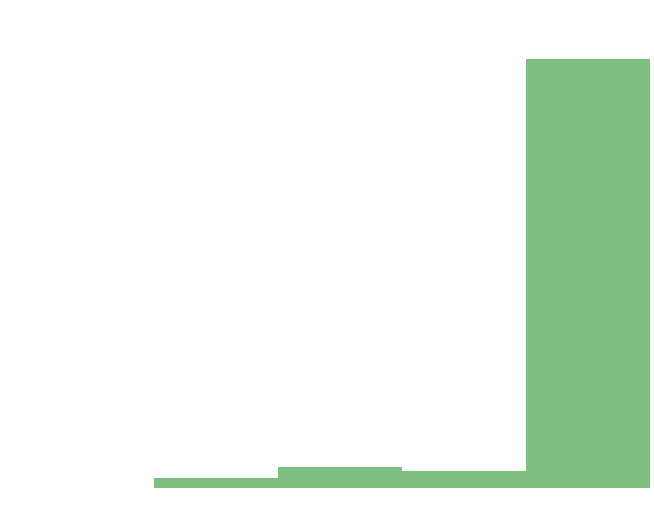
\includegraphics[width = 2cm, height = 0.5cm]{tex-inputs/data10/learnedyourusernameandpasswordforwebsitescombined}\\
8 & credit card information & 88.98\% & 0.56 & 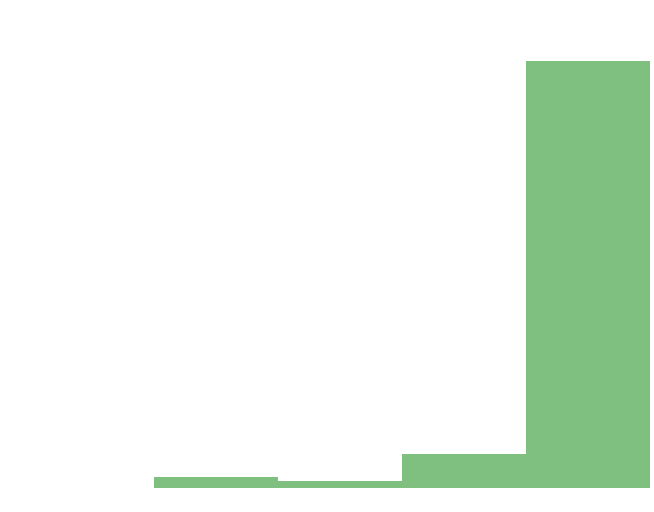
\includegraphics[width = 2cm, height = 0.5cm]{tex-inputs/data10/learnedyourcreditcardinformationcombined}\\
9 & video of you that is very embarrassing & 88.41\% & 0.53 & 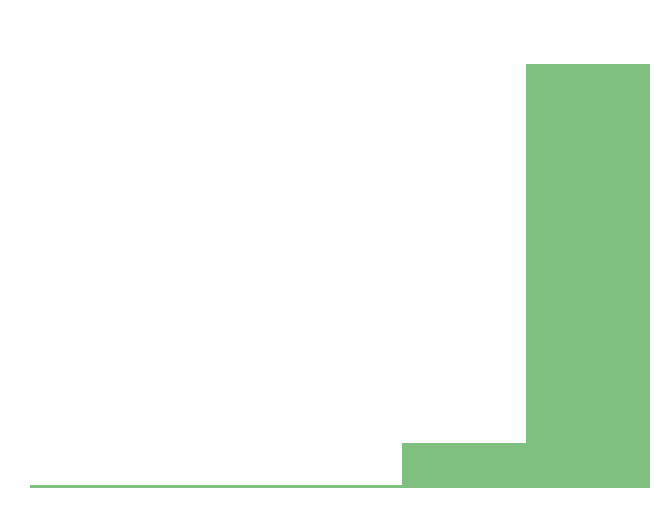
\includegraphics[width = 2cm, height = 0.5cm]{tex-inputs/data10/tookanincriminatingvideoofyoudoingsomethingembarrassingcombined}\\
10 & photo of you at home & 87.50\% & 0.60 & 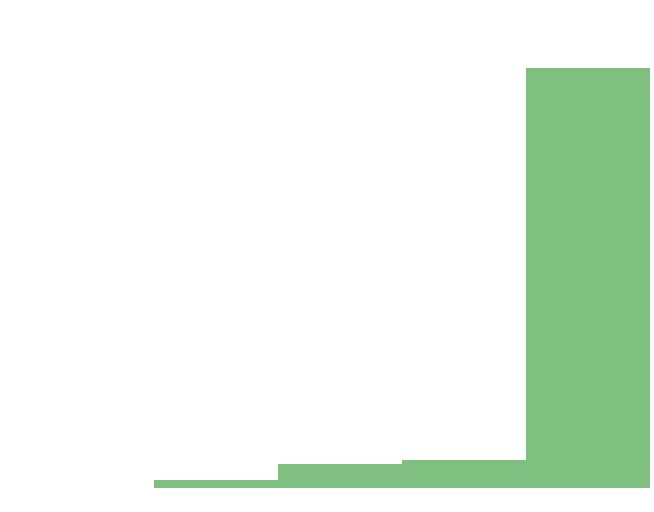
\includegraphics[width = 2cm, height = 0.5cm]{tex-inputs/data10/tookphotosofyou(withaninward-facingcamera)athomecombined}\\
 & \vdots & & & \\
64 & eye patterns (for eye tracking) & 40.51\%& 1.27 & 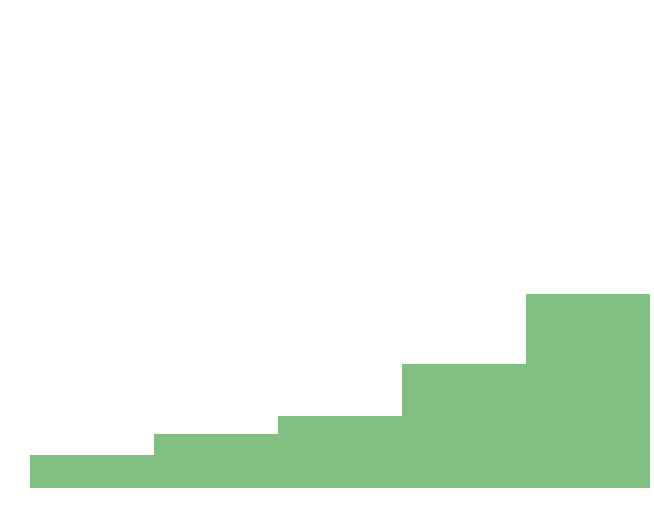
\includegraphics[width = 2cm, height = 0.5cm]{tex-inputs/data10/scannedyoureyetolearnyoureyepatterns(foreyetracking)combined} \\
65 & exercise patterns  & 38.66\% & 1.26 & 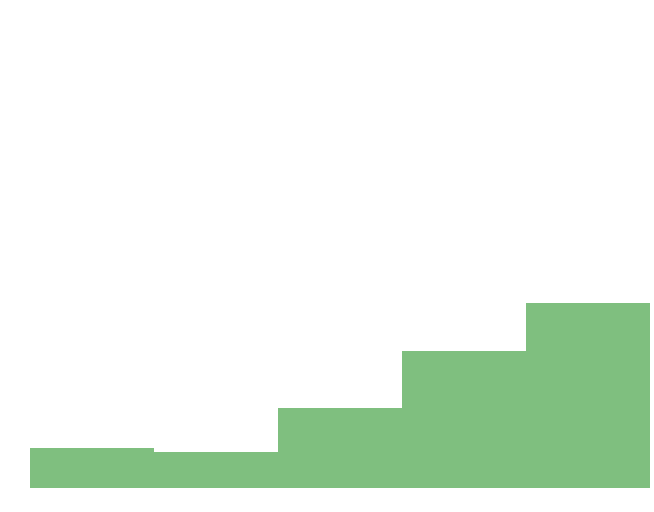
\includegraphics[width = 2cm, height = 0.5cm]{tex-inputs/data10/learnedwhenhowandhowmuchyouexercisecombined}\\
66 & when you are happy or having fun  & 34.75\% & 1.27 & 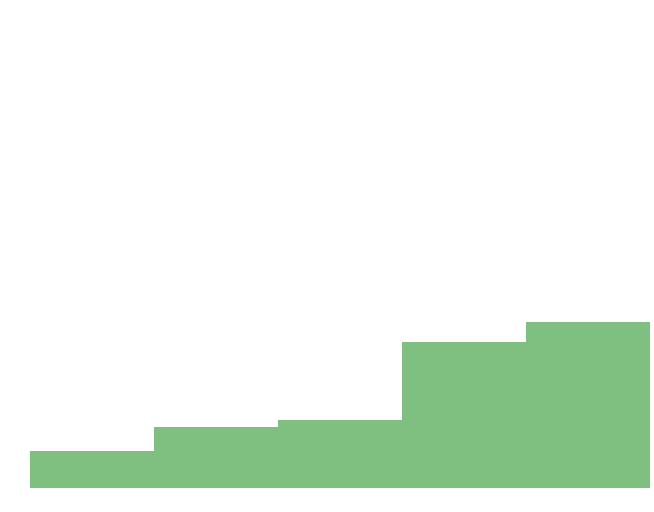
\includegraphics[width = 2cm, height = 0.5cm]{tex-inputs/data10/learnedwhenyouwerehappyorhavingfuncombined}\\
67 & television shows watched & 30.20\% & 1.40 & 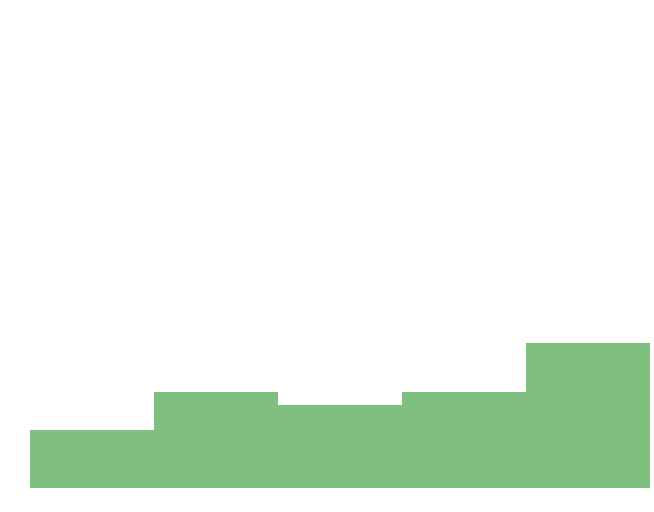
\includegraphics[width = 2cm, height = 0.5cm]{tex-inputs/data10/learnedwhattelevisionshowsyouwatchcombined}\\
68 & when you are busy or interruptible  & 29.50\% & 1.26 & 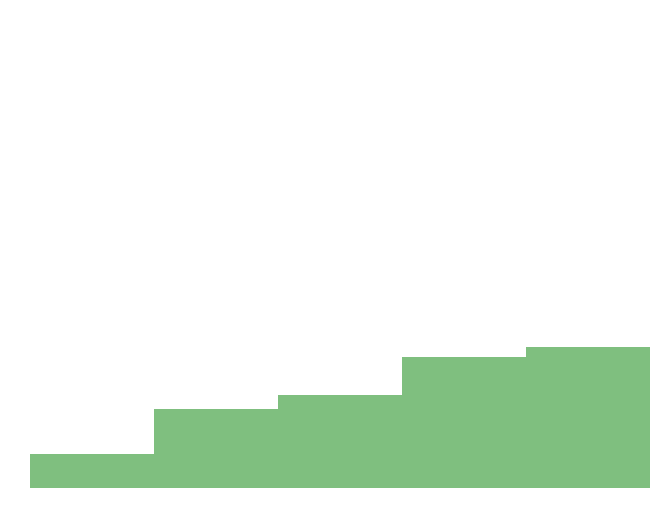
\includegraphics[width = 2cm, height = 0.5cm]{tex-inputs/data10/learnedwhenyouarebusyorinterruptiblecombined}\\
69 & music on device  & 28.06\% & 1.43 & 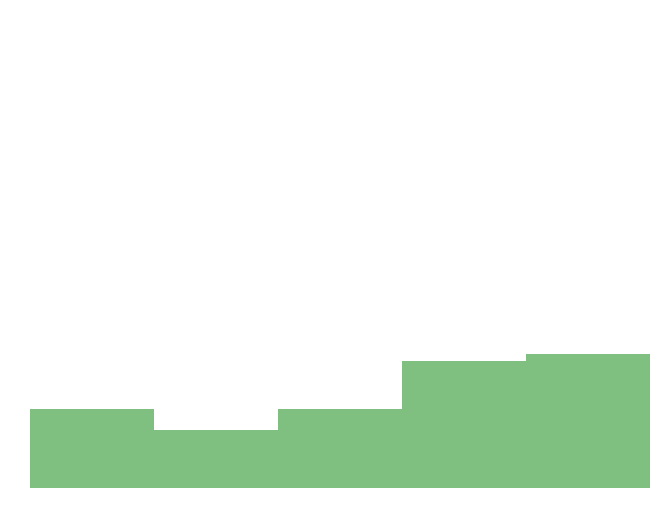
\includegraphics[width = 2cm, height = 0.5cm]{tex-inputs/data10/copiedanduploadedmusicfromyourdevicecombined}\\
70 & your heart rate & 27.50\% & 1.40 & 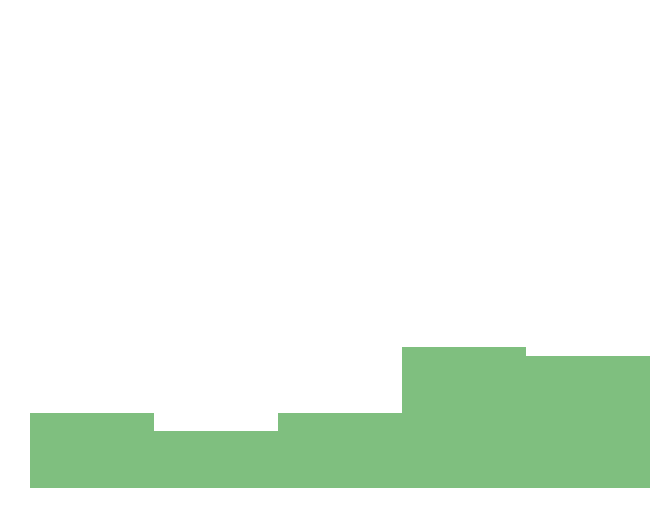
\includegraphics[width = 2cm, height = 0.5cm]{tex-inputs/data10/learnedyourheartratecombined} \\
71 & age & 24.29\% & 1.43 & 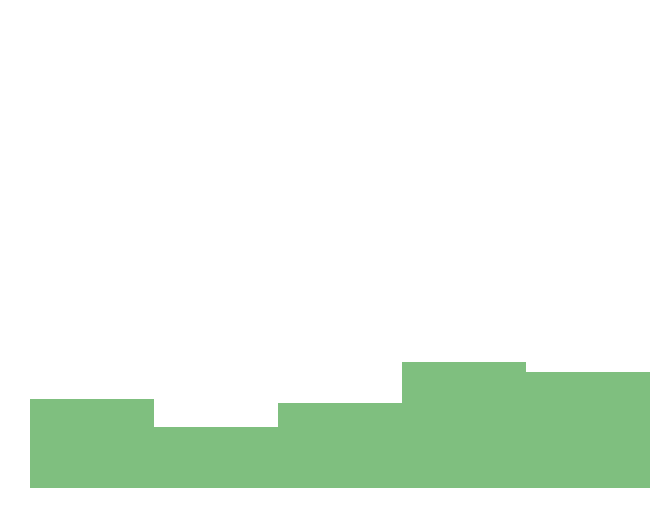
\includegraphics[width = 2cm, height = 0.5cm]{tex-inputs/data10/learnedyouragecombined}\\
72 & language spoken & 15.86\% & 1.49 & 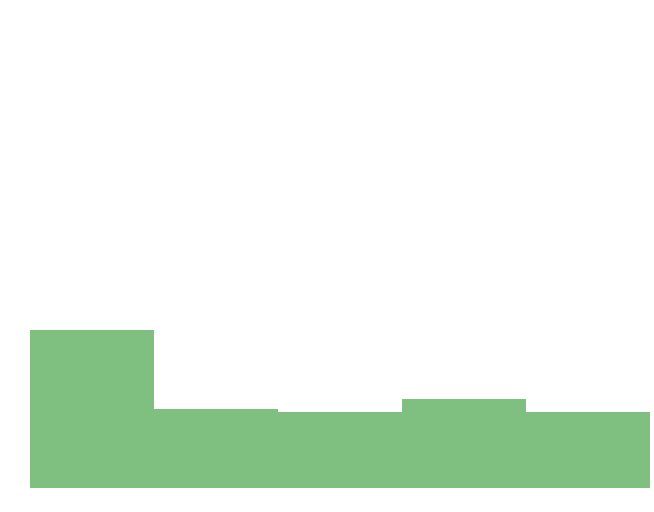
\includegraphics[width = 2cm, height = 0.5cm]{tex-inputs/data10/learnedthelanguageyouwerespeakingcombined}\\
73 & gender & 15.00\% & 1.45 & 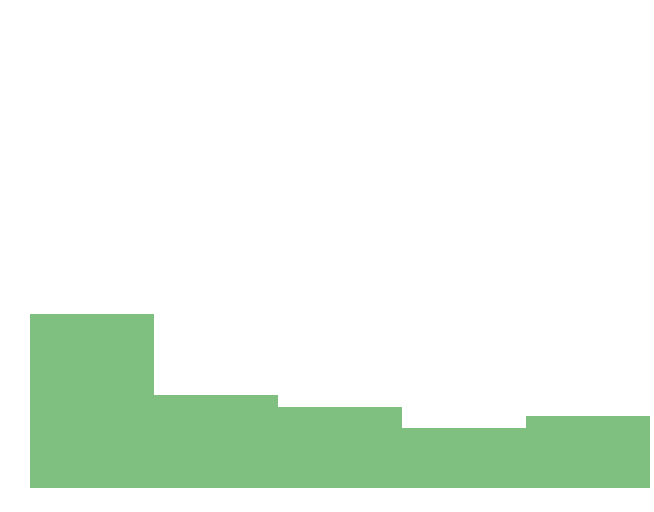
\includegraphics[width = 2cm, height = 0.5cm]{tex-inputs/data10/learnedyourgendercombined}\\ 
\hline
\end{tabular}
\caption{The 10 most and least upsetting data types, across all recipients. For the complete list of all data types across all recipients, see Appendix \ref{sec:data-appendix}.}
\label{top10-table}
\end{center}
\end{table*}


%A statistical analysis regarding the significance and confidence of <data> types with respect to all 72 was not performed due to the space constraints of the paper. We do consider all <data> categories in our statistical model, which provides an analysis of what factors had contributed to the perceived severity of a particular situation. 









